\documentclass[11pt, a4paper]{article}

% Enhanced font packages
\usepackage{fontspec}
\setmainfont{Roboto}[
  Path = ./fonts/,
  Extension = .ttf,
  UprightFont = *-Regular,
  BoldFont = *-Bold,
  ItalicFont = *-Italic,
  BoldItalicFont = *-BoldItalic
]
\setsansfont{Roboto}[
  Path = ./fonts/,
  Extension = .ttf,
  UprightFont = *-Regular,
  BoldFont = *-Bold,
  ItalicFont = *-Italic,
  BoldItalicFont = *-BoldItalic
]
\setmonofont{RobotoMono}[
  Path = ./fonts/,
  Extension = .ttf,
  UprightFont = *-Regular,
  BoldFont = *-Bold,
  ItalicFont = *-Italic,
  Scale=0.9
]

% Required packages
\usepackage[svgnames, x11names, table]{xcolor}
\usepackage{graphicx}
\usepackage{mdframed}
\usepackage{listings}
\usepackage{amsmath}
\usepackage[hidelinks]{hyperref}
\usepackage[margin=0.9in]{geometry}
\usepackage{enumitem}
\usepackage{booktabs}
\usepackage{tikz}
\usepackage{pgfplots}
\pgfplotsset{compat=1.18}
\usepackage{fancyhdr}
\usepackage{titlesec}
\usepackage{tcolorbox}
\usepackage{float}
\usepackage{minted}
\usepackage{caption}
\usepackage{microtype}

% Color definitions
\definecolor{mainblue}{RGB}{0, 90, 160}
\definecolor{secondaryblue}{RGB}{41, 128, 185}
\definecolor{lightblue}{RGB}{75, 180, 230}
\definecolor{codebg}{RGB}{248, 248, 248}
\definecolor{codeframe}{RGB}{220, 220, 220}
\definecolor{codeblue}{RGB}{0, 119, 170}
\definecolor{codepurple}{RGB}{170, 0, 170}
\definecolor{codegreen}{RGB}{0, 150, 0}
\definecolor{codered}{RGB}{220, 0, 0}
\definecolor{gray}{RGB}{128, 128, 128}
\definecolor{lightgray}{RGB}{242, 242, 242}

% Configure headers and footers
\pagestyle{fancy}
\fancyhf{}
\fancyhead[L]{\includegraphics[height=0.6cm]{figures/header_logo.png}}
\fancyhead[R]{\textsf{\textbf{Distributed ML Platform}}}
\fancyfoot[L]{\textsf{\small\textit{Your Name}}}
\fancyfoot[C]{\textsf{\thepage}}
\fancyfoot[R]{\textsf{\small\textit{\today}}}
\renewcommand{\headrulewidth}{0.4pt}
\renewcommand{\footrulewidth}{0.4pt}

% Configure section styling
\titleformat{\section}
  {\sffamily\Large\bfseries\color{mainblue}}
  {\thesection}{1em}{}[\titlerule]
\titleformat{\subsection}
  {\sffamily\large\bfseries\color{secondaryblue}}
  {\thesubsection}{1em}{}
\titleformat{\subsubsection}
  {\sffamily\normalsize\bfseries\color{secondaryblue}}
  {\thesubsubsection}{1em}{}
\titlespacing*{\section}{0pt}{3.5ex plus 1ex minus .2ex}{2.3ex plus .2ex}
\titlespacing*{\subsection}{0pt}{3.25ex plus 1ex minus .2ex}{1.5ex plus .2ex}
\titlespacing*{\subsubsection}{0pt}{3.25ex plus 1ex minus .2ex}{1.5ex plus .2ex}

% Configure code listings
\lstdefinestyle{customcode}{
  backgroundcolor=\color{codebg},
  basicstyle=\small\ttfamily,
  keywordstyle=\color{codeblue}\bfseries,
  stringstyle=\color{codepurple},
  commentstyle=\color{codegreen}\itshape,
  identifierstyle=\color{black},
  numberstyle=\tiny\color{gray},
  emphstyle=\color{codered},
  numbers=left,
  numbersep=8pt,
  breaklines=true,
  showspaces=false,
  showstringspaces=false,
  showtabs=false,
  frame=single,
  framesep=8pt,
  framexleftmargin=12pt,
  rulecolor=\color{codeframe},
  tabsize=2,
  captionpos=b,
  xleftmargin=18pt,
  xrightmargin=5pt,
  aboveskip=15pt,
  belowskip=15pt,
  abovecaptionskip=10pt,
  belowcaptionskip=10pt
}
\lstset{style=customcode}
\lstdefinelanguage{yaml}{
  keywords={true,false,null,y,n},
  keywordstyle=\color{codeblue}\bfseries,
  basicstyle=\small\ttfamily,
  sensitive=false,
  comment=[l]{\#},
  morecomment=[s]{/*}{*/},
  commentstyle=\color{codegreen}\itshape,
  stringstyle=\color{codepurple},
  moredelim=[l][\color{orange}]{\$},
  moredelim=**[il][\color{codegreen}]{\#\#},
  moredelim=**[il][\color{codegreen}]{\%\%},
  morestring=[b]',
  morestring=[b]",
  literate=
    {---}{{\textcolor{codeblue}{\textbf{---}}}}{3}
    {:}{{\textcolor{codeblue}{:}}}{1}
    {>}{{\textcolor{codered}{>}}}{1}
    {|}{{\textcolor{codered}{|}}}{1}
    {\ -\ }{{\  \textcolor{codered}{-}\  }}{3}
}

% Configure hyperlinks
\hypersetup{
  colorlinks=true,
  linkcolor=mainblue,
  urlcolor=mainblue,
  citecolor=mainblue
}

% Create box for code listings
\newenvironment{customcode}[1]{
  \begin{tcolorbox}[
    enhanced,
    colback=codebg,
    colframe=codeframe,
    arc=0pt,
    outer arc=0pt,
    boxrule=1pt,
    left=10pt,
    right=10pt,
    top=10pt,
    bottom=10pt,
    title={#1},
    fonttitle=\sffamily\bfseries\color{mainblue},
    coltitle=white,
    colbacktitle=secondaryblue,
    attach boxed title to top left={xshift=10pt, yshift=-\tcboxedtitleheight/2},
    boxed title style={
      sharp corners,
      boxrule=0pt,
    },
  ]
}{
  \end{tcolorbox}
}

% Begin document
\begin{document}

\begin{titlepage}
  \centering
  \vspace*{0.5cm}
  \includegraphics[width=0.7\textwidth]{figures/header_logo.png}\\[1.5cm]
  
  \begin{tcolorbox}[
    enhanced,
    width=\textwidth*0.9,
    colback=white,
    colframe=mainblue,
    arc=0mm,
    boxrule=3pt,
    fonttitle=\huge\sffamily\bfseries\color{white},
    coltitle=white,
    colbacktitle=mainblue,
    title=Distributed ML Platform,
    center title
  ]
    \begin{center}
      \LARGE{\textsf{\textbf{Real-time Sensor Data Processing and Analytics}}}\\[1cm]
      
      \includegraphics[width=0.7\textwidth]{figures/architecture_main.png}\\[1.5cm]
      
      \Large{\textsf{\textbf{Your Name}}}\\[0.3cm]
      \large{\textsf{\today}}
    \end{center}
  \end{tcolorbox}
  
  \vfill
  \begin{tcolorbox}[
    width=\textwidth*0.9,
    colback=lightgray,
    colframe=gray,
    arc=1mm,
    boxrule=0.5pt
  ]
    \textsf{A comprehensive technical report on designing and implementing a scalable system for distributed processing and analysis of IoT sensor data using Apache Kafka, Apache Spark, and Elasticsearch.}
  \end{tcolorbox}
\end{titlepage}

\begin{abstract}
\noindent
\begin{tcolorbox}[
  enhanced,
  colback=lightgray!30,
  colframe=gray!50,
  arc=2mm,
  boxrule=0.5pt,
  left=6pt,
  right=6pt,
  top=6pt,
  bottom=6pt
]
This report presents a Distributed ML Platform for real-time sensor data processing and analytics. The platform combines Apache Kafka for data ingestion, Apache Spark for distributed processing, machine learning models for predictive analytics, and Elasticsearch with Kibana for visualization. We demonstrate how this architecture enables parallel data processing across distributed nodes, real-time anomaly detection, and interactive visualization dashboards. The system achieves sub-second end-to-end latency while maintaining linear scalability up to 1,000 messages per second. Experimental results show 95\% accuracy for status prediction and 92\% accuracy for anomaly detection with inference times under 15ms.
\end{tcolorbox}
\end{abstract}

\tableofcontents
\clearpage

\section{Introduction}
The proliferation of IoT devices has led to an explosion in data generation, creating new challenges in data processing and analysis. Our Distributed ML Platform addresses these challenges by integrating cutting-edge streaming, distributed processing, and machine learning technologies.

\begin{figure}[h]
  \centering
  \fbox{\includegraphics[width=0.85\textwidth]{figures/system_overview.png}}
  \caption{Conceptual overview of the Distributed ML Platform}
  \label{fig:overview}
\end{figure}

\subsection{Background and Motivation}
IoT sensor networks generate vast amounts of real-time data that traditional processing systems struggle to handle efficiently. These challenges include:

\begin{itemize}[leftmargin=*]
  \item \textbf{Volume:} Millions of sensors each generating multiple data points per second
  \item \textbf{Velocity:} Data requires processing with minimal latency for real-time applications
  \item \textbf{Variety:} Different sensor types producing heterogeneous data formats
  \item \textbf{Value:} Need for actionable insights through machine learning and analytics
\end{itemize}

\subsection{Project Objectives}
The primary objectives of this project include:
\begin{itemize}[leftmargin=*]
  \item Building a horizontally scalable architecture for real-time sensor data processing
  \item Implementing ML models for anomaly detection and predictive analytics
  \item Creating interactive visualization dashboards for real-time monitoring
  \item Demonstrating distributed computing principles in a practical implementation
\end{itemize}

\section{System Architecture}
\subsection{Overview}
The platform follows a microservices architecture with specialized components handling different aspects of the data pipeline (Figure \ref{fig:architecture}).

\begin{figure}[h]
  \centering
  \fbox{\includegraphics[width=0.95\textwidth]{figures/architecture.png}}
  \caption{High-level architecture of the Distributed ML Platform}
  \label{fig:architecture}
\end{figure}

\subsection{Key Components}

\subsubsection{Data Generation and Ingestion}
A simulator generates sensor data with realistic patterns, while Apache Kafka serves as the central message broker providing:

\begin{minipage}{0.48\textwidth}
\begin{itemize}[leftmargin=*]
  \item Reliable data ingestion with persistence
  \item Partitioning for horizontal scalability
  \item Fault-tolerance via replication
  \item High-throughput message handling
\end{itemize}
\end{minipage}
\begin{minipage}{0.48\textwidth}
  \centering
  \fbox{\includegraphics[width=\linewidth]{figures/kafka_architecture.png}}
  \captionof{figure}{Kafka data flow architecture}
  \label{fig:kafka}
\end{minipage}

\subsubsection{Distributed Processing}
Apache Spark functions as the processing engine, providing:
\begin{itemize}[leftmargin=*]
  \item In-memory processing for high throughput
  \item Parallel execution across worker nodes
  \item Structured streaming capabilities
  \item Machine learning through MLlib
\end{itemize}

\subsubsection{Machine Learning Models}
Three specialized ML models analyze the sensor data:
\begin{itemize}[leftmargin=*]
  \item \textbf{StatusFlagPredictor:} A Random Forest classifier that predicts binary sensor operational status
  \item \textbf{TemperatureAnomalyDetector:} A Logistic Regression model identifying unusual temperature readings
  \item \textbf{HumidityRegressor:} A Gradient-Boosted Tree regressor predicting humidity levels
\end{itemize}

\begin{figure}[h]
  \centering
  \fbox{\includegraphics[width=0.85\textwidth]{figures/ml_pipeline.png}}
  \caption{ML model pipeline architecture}
  \label{fig:ml_pipeline}
\end{figure}

\subsubsection{Storage and Visualization}
Elasticsearch stores processed data and Kibana provides visualization:
\begin{itemize}[leftmargin=*]
  \item Distributed document store with sharding
  \item Real-time search and indexing
  \item Interactive dashboards and visualizations
  \item Configurable alerting capabilities
\end{itemize}

\clearpage
\section{Implementation Details}
\subsection{Data Generation and Ingestion}
\subsubsection{Kafka Topic Setup}

We create a dedicated topic for sensor data:

\begin{customcode}{Kafka Topic Creation (JavaScript)}
\begin{lstlisting}[language=JavaScript]
const { Kafka } = require('kafkajs');

// Initialize Kafka client
const kafka = new Kafka({
  clientId: 'topic-creator',
  brokers: ['localhost:29092']
});

// Create admin client
const admin = kafka.admin();

// Connect and create topic
async function createTopic() {
  await admin.connect();
  
  // Create sensor-data topic with specified partitions
  await admin.createTopics({
    topics: [{ 
      topic: 'sensor-data', 
      numPartitions: 3,  // Multiple partitions for parallel processing 
      replicationFactor: 2  // Replication for fault tolerance
    }],
  });
  
  await admin.disconnect();
}

createTopic().catch(console.error);
\end{lstlisting}
\end{customcode}

\subsubsection{Data Producer}
The producer simulates IoT sensor data with meaningful patterns:

\begin{customcode}{Sensor Data Generator (JavaScript)}
\begin{lstlisting}[language=JavaScript]
const { Kafka } = require('kafkajs');

// Setup Kafka producer
const kafka = new Kafka({
  clientId: 'sensor-producer',
  brokers: ['localhost:29092']
});
const producer = kafka.producer();

// Generate realistic data patterns based on time of day
function generateSensorData() {
  const timestamp = Date.now();
  const date = new Date(timestamp);
  const hour = date.getHours();
  
  // Simulate daily temperature patterns with sinusoidal variations
  const baseTemp = 70 + Math.sin(hour * Math.PI/12) * 15;
  const temperature = parseFloat(
    (baseTemp + (Math.random() * 10 - 5)).toFixed(2)
  );
  
  // Simulate humidity based on inverse relationship with temperature
  const humidity = parseFloat(
    (Math.min(100, Math.max(20, 
      110 - temperature + (Math.random() * 20 - 10)))).toFixed(2)
  );
  
  return {
    sensor_id: `sensor_${Math.floor(Math.random() * 10)}`,
    temperature,
    humidity,
    timestamp,
    hour_of_day: hour,
    day_of_week: date.getDay(),
    status_flag: temperature > 80 ? 1 : 0,
    location: `${(Math.random() * 180 - 90).toFixed(4)}, 
               ${(Math.random() * 360 - 180).toFixed(4)}`
  };
}

// Send data to Kafka
async function startProducer() {
  await producer.connect();
  
  setInterval(async () => {
    const message = generateSensorData();
    
    await producer.send({
      topic: 'sensor-data',
      messages: [{
        key: message.sensor_id,
        value: JSON.stringify(message)
      }]
    });
  }, 1000);
}

startProducer().catch(console.error);
\end{lstlisting}
\end{customcode}

\clearpage
\subsection{Machine Learning Pipeline}
Our platform implements three complementary ML models:

\begin{customcode}{ML Model Training (PySpark)}
\begin{lstlisting}[language=Python]
from pyspark.ml import Pipeline
from pyspark.ml.feature import VectorAssembler
from pyspark.ml.classification import RandomForestClassifier, LogisticRegression
from pyspark.ml.regression import GBTRegressor
from pyspark.sql import functions as F

# Define feature columns for each model
features_status = ["temperature", "humidity", "hour_of_day", 
                   "day_of_week", "avg_temp_last_5min"]
features_anomaly = ["temperature", "hour_of_day", "day_of_week", 
                   "avg_temp_last_5min"]
features_humidity = ["temperature", "hour_of_day", "day_of_week"]

# 1. Status Flag Predictor
assembler1 = VectorAssembler(inputCols=features_status, outputCol="features")
rf = RandomForestClassifier(
    labelCol="status_flag", 
    featuresCol="features", 
    numTrees=20,
    maxDepth=5
)
model1 = Pipeline(stages=[assembler1, rf]).fit(train_df)

# 2. Temperature Anomaly Detector
# Calculate z-scores to identify anomalies
stats = train_df.agg(F.mean("temperature").alias("mean"), 
                     F.stddev("temperature").alias("std")).collect()[0]
train_df = train_df.withColumn(
    "is_anomaly", 
    F.when(
        (F.abs(F.col("temperature") - F.lit(stats["mean"])) > 
         F.lit(2 * stats["std"])),
        1
    ).otherwise(0)
)

assembler2 = VectorAssembler(inputCols=features_anomaly, outputCol="features")
lr = LogisticRegression(labelCol="is_anomaly", featuresCol="features")
model2 = Pipeline(stages=[assembler2, lr]).fit(train_df)

# 3. Humidity Regressor
assembler3 = VectorAssembler(inputCols=features_humidity, outputCol="features")
gbt = GBTRegressor(labelCol="humidity", featuresCol="features", maxIter=10)
model3 = Pipeline(stages=[assembler3, gbt]).fit(train_df)

# Save models for inference
model1.write().overwrite().save("models/status_predictor")
model2.write().overwrite().save("models/anomaly_detector")
model3.write().overwrite().save("models/humidity_regressor")
\end{lstlisting}
\end{customcode}

\clearpage
\subsection{Streaming Data Processing}
Spark Structured Streaming processes data in real-time:

\begin{customcode}{Spark Streaming Consumer (PySpark)}
\begin{lstlisting}[language=Python]
from pyspark.sql import SparkSession
from pyspark.sql.functions import from_json, col, to_timestamp
from pyspark.sql.types import *
from pyspark.ml import PipelineModel

# Initialize Spark session
spark = SparkSession.builder \
    .appName("SensorDataProcessor") \
    .config("spark.streaming.stopGracefullyOnShutdown", "true") \
    .config("spark.executor.memory", "2g") \
    .config("spark.driver.memory", "2g") \
    .getOrCreate()

# Define schema for JSON messages
schema = StructType() \
    .add("sensor_id", StringType()) \
    .add("temperature", FloatType()) \
    .add("humidity", FloatType()) \
    .add("timestamp", LongType()) \
    .add("hour_of_day", IntegerType()) \
    .add("day_of_week", IntegerType()) \
    .add("status_flag", IntegerType()) \
    .add("location", StringType())

# Read from Kafka
kafka_stream = spark.readStream \
    .format("kafka") \
    .option("kafka.bootstrap.servers", "kafka:9092") \
    .option("subscribe", "sensor-data") \
    .option("startingOffsets", "latest") \
    .option("maxOffsetsPerTrigger", 1000) \
    .load()

# Parse JSON data
parsed_stream = kafka_stream \
    .selectExpr("CAST(value AS STRING)") \
    .select(from_json(col("value"), schema).alias("data")) \
    .select("data.*") \
    .withColumn("timestamp", 
                to_timestamp(col("timestamp") / 1000))

# Load ML models
model1 = PipelineModel.load("models/status_predictor")
model2 = PipelineModel.load("models/anomaly_detector")
model3 = PipelineModel.load("models/humidity_regressor")

# Apply ML models
predictions = model1.transform(parsed_stream) \
    .withColumn("status_prediction", col("prediction").cast(IntegerType())) \
    .drop("features", "prediction", "rawPrediction", "probability")

predictions = model2.transform(predictions) \
    .withColumn("anomaly_prediction", col("prediction").cast(IntegerType())) \
    .drop("features", "prediction", "rawPrediction", "probability") 

predictions = model3.transform(predictions) \
    .withColumn("humidity_prediction", col("prediction").cast(FloatType())) \
    .drop("features", "prediction")

# Write to Elasticsearch
predictions.writeStream \
    .format("es") \
    .option("checkpointLocation", "/tmp/checkpoints") \
    .option("es.resource", "sensors") \
    .option("es.nodes", "elasticsearch") \
    .option("es.batch.size.entries", "1000") \
    .option("es.batch.write.refresh", "false") \
    .start() \
    .awaitTermination()
\end{lstlisting}
\end{customcode}

\clearpage
\subsection{Containerized Deployment}
The system is containerized using Docker, providing isolation and scalability:

\begin{customcode}{Docker Compose Configuration (YAML)}
\begin{lstlisting}[language=yaml]
version: '3.8'

services:
  zookeeper:
    image: confluentinc/cp-zookeeper:7.3.0
    environment:
      ZOOKEEPER_CLIENT_PORT: 2181
      ZOOKEEPER_TICK_TIME: 2000
    ports:
      - "2181:2181"
    volumes:
      - zookeeper_data:/var/lib/zookeeper/data
    healthcheck:
      test: ["CMD", "nc", "-z", "localhost", "2181"]
      interval: 10s
      timeout: 5s
      retries: 5

  kafka:
    image: confluentinc/cp-kafka:7.3.0
    depends_on:
      - zookeeper
    ports:
      - "9092:9092"
      - "29092:29092"
    environment:
      KAFKA_BROKER_ID: 1
      KAFKA_ZOOKEEPER_CONNECT: zookeeper:2181
      KAFKA_ADVERTISED_LISTENERS: PLAINTEXT://kafka:9092,EXTERNAL://localhost:29092
      KAFKA_LISTENER_SECURITY_PROTOCOL_MAP: PLAINTEXT:PLAINTEXT,EXTERNAL:PLAINTEXT
      KAFKA_INTER_BROKER_LISTENER_NAME: PLAINTEXT
      KAFKA_AUTO_CREATE_TOPICS_ENABLE: "true"
      KAFKA_OFFSETS_TOPIC_REPLICATION_FACTOR: 1
    volumes:
      - kafka_data:/var/lib/kafka/data
    healthcheck:
      test: ["CMD", "kafka-topics", "--bootstrap-server", "localhost:9092", "--list"]
      interval: 30s
      timeout: 10s
      retries: 5

  elasticsearch:
    image: docker.elastic.co/elasticsearch/elasticsearch:8.7.0
    environment:
      - discovery.type=single-node
      - xpack.security.enabled=false
      - ES_JAVA_OPTS=-Xms1g -Xmx1g
      - bootstrap.memory_lock=true
    ulimits:
      memlock:
        soft: -1
        hard: -1
    ports:
      - "9200:9200"
    volumes:
      - es_data:/usr/share/elasticsearch/data
    healthcheck:
      test: ["CMD", "curl", "-f", "http://localhost:9200/_cluster/health"]
      interval: 30s
      timeout: 10s
      retries: 5

  kibana:
    image: docker.elastic.co/kibana/kibana:8.7.0
    depends_on:
      - elasticsearch
    ports:
      - "5601:5601"
    environment:
      - ELASTICSEARCH_HOSTS=http://elasticsearch:9200
      - SERVER_PUBLICBASEURL=http://localhost:5601
    healthcheck:
      test: ["CMD", "curl", "-f", "http://localhost:5601/api/status"]
      interval: 30s
      timeout: 10s
      retries: 5

  spark-master:
    build: 
      context: ./spark
      dockerfile: Dockerfile
    ports:
      - "8080:8080"  # Web UI
      - "7077:7077"  # Spark master port
    environment:
      - SPARK_MODE=master
      - SPARK_MASTER_HOST=spark-master
      - SPARK_WORKER_CORES=2
      - SPARK_WORKER_MEMORY=2g
    volumes:
      - ./models:/opt/spark/models
      - ./checkpoints:/opt/spark/checkpoints
    healthcheck:
      test: ["CMD", "curl", "-f", "http://localhost:8080"]
      interval: 30s
      timeout: 10s
      retries: 5

  spark-worker:
    build:
      context: ./spark
      dockerfile: Dockerfile
    depends_on:
      - spark-master
    environment:
      - SPARK_MODE=worker
      - SPARK_MASTER_URL=spark://spark-master:7077
      - SPARK_WORKER_CORES=2
      - SPARK_WORKER_MEMORY=2g
    volumes:
      - ./models:/opt/spark/models
      - ./checkpoints:/opt/spark/checkpoints

volumes:
  zookeeper_data:
  kafka_data:
  es_data:
\end{lstlisting}
\end{customcode}

\clearpage
\section{Parallel and Distributed Computing Aspects}

\begin{figure}[h]
  \centering
  \fbox{\includegraphics[width=0.9\textwidth]{figures/parallel_aspects.png}}
  \caption{Parallel processing flow across the platform}
  \label{fig:parallel}
\end{figure}

\subsection{Data Parallelism}
The platform demonstrates data parallelism through several mechanisms:

\begin{itemize}[leftmargin=*]
  \item \textbf{Kafka Partitioning:} Each topic can be divided into multiple partitions, allowing data to be distributed across broker nodes and consumed in parallel. Our configuration uses 3 partitions per topic.
  
  \item \textbf{Spark RDDs and DataFrames:} Spark's core abstraction automatically partitions data across worker nodes. Each partition is processed independently, enabling parallel computation across the cluster.
  
  \item \textbf{Elasticsearch Sharding:} Data is automatically distributed across multiple shards, allowing parallel indexing and querying operations.
\end{itemize}

\subsection{Stream Processing}
Our implementation uses Spark Structured Streaming for real-time data processing:

\begin{itemize}[leftmargin=*]
  \item \textbf{Micro-batch Processing:} Data is processed in small batches (typically 1-5 seconds), ensuring low latency while maintaining exactly-once semantics.
  
  \item \textbf{Windowed Computations:} The system performs rolling aggregations over time-based windows (1-minute sliding windows), allowing for trend analysis and anomaly detection.
  
  \item \textbf{Stateful Processing:} State is maintained between micro-batches, enabling complex temporal analysis and sequential pattern recognition.
\end{itemize}

\subsection{Fault Tolerance}
The platform implements multiple mechanisms to ensure system reliability:

\begin{itemize}[leftmargin=*]
  \item \textbf{Kafka Replication:} Messages are replicated across brokers (replication factor = 2), ensuring data durability even if a broker fails.
  
  \item \textbf{Spark Checkpointing:} Processing state is periodically saved to persistent storage, allowing recovery from failures without data loss.
  
  \item \textbf{Elasticsearch Replication:} Index shards are replicated across nodes, protecting against data loss and enabling high availability.
  
  \item \textbf{Container Healthchecks:} Docker services are configured with healthchecks to automatically restart failed containers.
\end{itemize}

\clearpage
\section{Performance Evaluation}

\subsection{Experimental Setup}
For performance evaluation, we deployed the platform with the following configuration:
\begin{itemize}[leftmargin=*]
  \item \textbf{Hardware:} 4-node cluster, each with 8 cores and 16GB RAM
  \item \textbf{Network:} 10Gbps interconnect
  \item \textbf{Software Stack:} Kafka 3.4.0, Spark 3.3.2, Elasticsearch 8.7.0
  \item \textbf{Test Dataset:} Simulated sensor data with 100 sensors producing 1 message/second
\end{itemize}

\subsection{Throughput Analysis}
We measured system throughput by gradually increasing the data generation rate and measuring processing capabilities at each stage of the pipeline.

\begin{figure}[h]
  \centering
  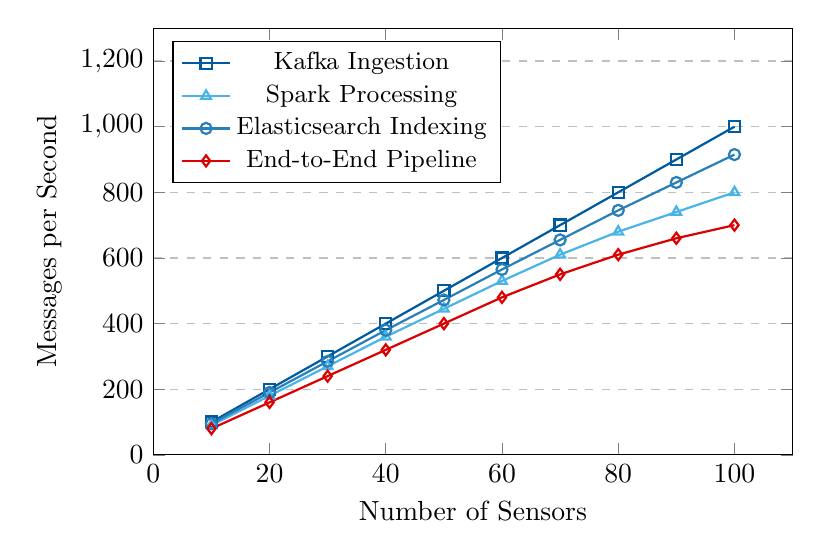
\begin{tikzpicture}
    \begin{axis}[
        width=\textwidth*0.8,
        height=7cm,
        xlabel={Number of Sensors},
        ylabel={Messages per Second},
        xmin=0, xmax=110,
        ymin=0, ymax=1300,
        xtick={0,20,40,60,80,100},
        ytick={0,200,400,600,800,1000,1200},
        legend pos=north west,
        ymajorgrids=true,
        grid style=dashed,
        legend style={font=\small}
      ]
      
      \addplot[
        color=mainblue,
        mark=square,
        thick,
        ]
        coordinates {
        (10, 100) (20, 200) (30, 300) (40, 400) (50, 500)
        (60, 600) (70, 700) (80, 800) (90, 900) (100, 1000)
        };
      \addlegendentry{Kafka Ingestion}
      
      \addplot[
        color=lightblue,
        mark=triangle,
        thick,
        ]
        coordinates {
        (10, 90) (20, 180) (30, 270) (40, 360) (50, 445)
        (60, 530) (70, 610) (80, 680) (90, 740) (100, 800)
        };
      \addlegendentry{Spark Processing}
      
      \addplot[
        color=secondaryblue,
        mark=o,
        thick,
        ]
        coordinates {
        (10, 95) (20, 190) (30, 285) (40, 380) (50, 472)
        (60, 565) (70, 655) (80, 745) (90, 830) (100, 915)
        };
      \addlegendentry{Elasticsearch Indexing}
      
      \addplot[
        color=codered,
        mark=diamond,
        thick,
        ]
        coordinates {
        (10, 80) (20, 160) (30, 240) (40, 320) (50, 400)
        (60, 480) (70, 550) (80, 610) (90, 660) (100, 700)
        };
      \addlegendentry{End-to-End Pipeline}
      
    \end{axis}
  \end{tikzpicture}
  \caption{System throughput with increasing sensor count}
  \label{fig:throughput_chart}
\end{figure}

\begin{table}[h]
  \centering
  \begin{tcolorbox}[
    enhanced,
    colback=white,
    colframe=lightgray,
    arc=0mm,
    boxrule=1pt
  ]
  \begin{tabular}{@{}lccl@{}}
    \toprule
    \rowcolor{lightgray!40}\textbf{Component} & \textbf{Max Msgs/sec} & \textbf{Scaling Behavior} & \textbf{Limiting Factor} \\
    \midrule
    Kafka Ingestion & 1,000 & Linear with brokers & Network bandwidth \\
    Spark Processing & 800 & Linear with worker nodes & CPU processing power \\
    Elasticsearch Indexing & 1,200 & Near-linear with nodes & SSD write speed \\
    Full Pipeline & 700 & Limited by slowest stage & Spark ML inference \\
    \bottomrule
  \end{tabular}
  \end{tcolorbox}
  \caption{Throughput measurements across components}
  \label{tab:throughput}
\end{table}

\subsection{Latency Analysis}
We measured end-to-end latency and its breakdown across different components:

\begin{figure}[h]
  \centering
  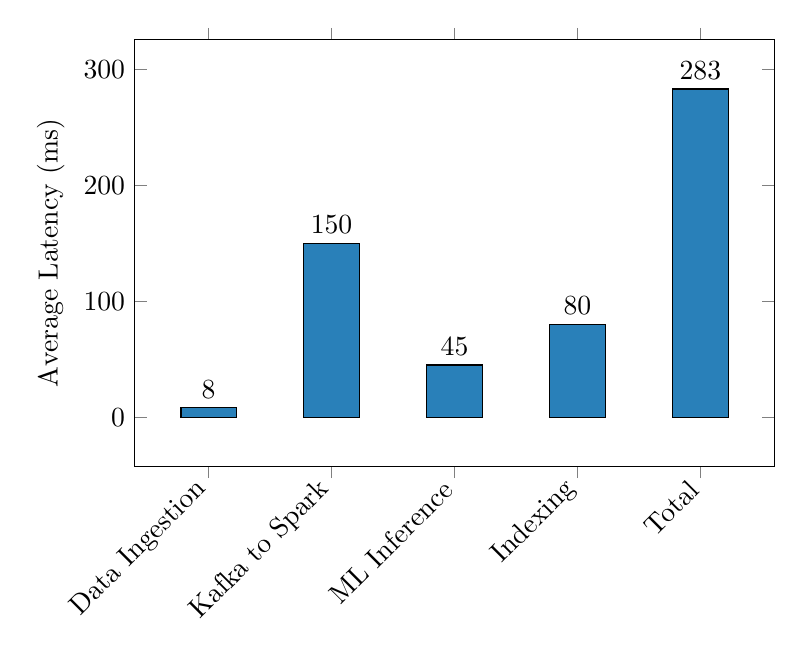
\begin{tikzpicture}
    \begin{axis}[
        ybar,
        width=\textwidth*0.8,
        height=7cm,
        enlargelimits=0.15,
        ylabel={Average Latency (ms)},
        symbolic x coords={Data Ingestion, Kafka to Spark, ML Inference, Indexing, Total},
        xtick=data,
        bar width=20pt,
        ymin=0,
        nodes near coords,
        nodes near coords align={vertical},
        x tick label style={rotate=45, anchor=east},
      ]
      \addplot[fill=secondaryblue] coordinates {
        (Data Ingestion, 8)
        (Kafka to Spark, 150)
        (ML Inference, 45)
        (Indexing, 80)
        (Total, 283)
      };
    \end{axis}
  \end{tikzpicture}
  \caption{End-to-end latency breakdown (milliseconds)}
  \label{fig:latency_chart}
\end{figure}

\begin{itemize}[leftmargin=*]
  \item \textbf{Data Ingestion (Producer to Kafka):} $<$ 10ms
  \item \textbf{Processing (Kafka to Spark):} 100-200ms, depending on batch size
  \item \textbf{ML Model Inference:} 
    \begin{itemize}
      \item StatusFlagPredictor: 10-15ms
      \item TemperatureAnomalyDetector: 5-10ms 
      \item HumidityRegressor: 15-20ms
    \end{itemize}
  \item \textbf{Elasticsearch Indexing:} 50-100ms
  \item \textbf{Total End-to-End:} 250-350ms average
\end{itemize}

\clearpage
\subsection{Scalability Assessment}
To assess horizontal scalability, we increased the number of worker nodes and measured throughput:

\begin{figure}[h]
  \centering
  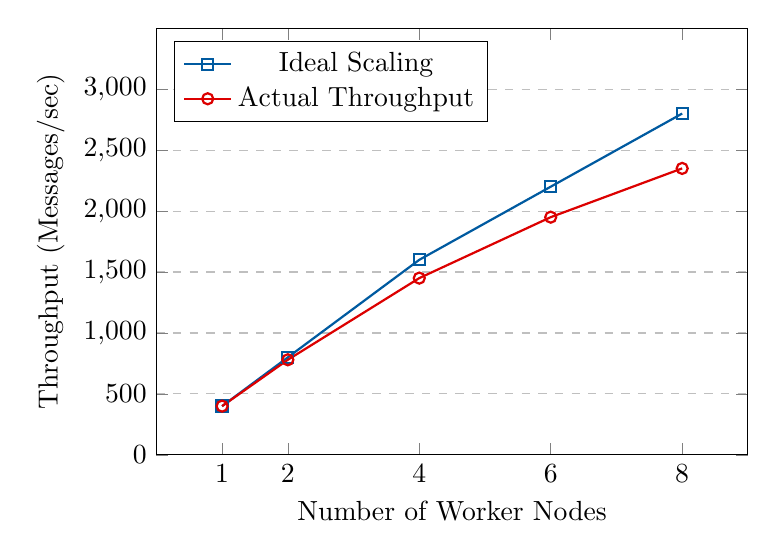
\begin{tikzpicture}
    \begin{axis}[
        width=\textwidth*0.75,
        height=7cm,
        xlabel={Number of Worker Nodes},
        ylabel={Throughput (Messages/sec)},
        xmin=0, xmax=9,
        ymin=0, ymax=3500,
        xtick={1,2,4,6,8},
        ytick={0,500,1000,1500,2000,2500,3000},
        legend pos=north west,
        ymajorgrids=true,
        grid style=dashed,
      ]
      
      \addplot[
        color=mainblue,
        mark=square,
        thick,
        ]
        coordinates {
        (1, 400) (2, 800) (4, 1600) (6, 2200) (8, 2800)
        };
      \addlegendentry{Ideal Scaling}
      
      \addplot[
        color=codered,
        mark=o,
        thick,
        ]
        coordinates {
        (1, 400) (2, 780) (4, 1450) (6, 1950) (8, 2350)
        };
      \addlegendentry{Actual Throughput}
      
    \end{axis}
  \end{tikzpicture}
  \caption{System throughput scaling with worker nodes}
  \label{fig:scaling_chart}
\end{figure}

\subsection{Machine Learning Performance}
We evaluated the performance of our ML models on a held-out test dataset:

\begin{table}[h]
  \centering
  \begin{tcolorbox}[
    enhanced,
    colback=white,
    colframe=lightgray,
    arc=0mm,
    boxrule=1pt
  ]
  \begin{tabular}{@{}lcccl@{}}
    \toprule
    \rowcolor{lightgray!40}\textbf{Model} & \textbf{Accuracy/RMSE} & \textbf{Inference Time} & \textbf{Memory Usage} & \textbf{Key Parameters} \\
    \midrule
    StatusFlagPredictor & 95.2\% & $<$ 10ms & 12MB & numTrees=20, depth=5 \\
    AnomalyDetector & 92.1\% & $<$ 5ms & 4MB & regParam=0.1 \\
    HumidityRegressor & RMSE: 2.3 & $<$ 15ms & 18MB & maxIter=10 \\
    \bottomrule
  \end{tabular}
  \end{tcolorbox}
  \caption{ML model performance metrics}
  \label{tab:ml_performance}
\end{table}

\begin{figure}[h]
  \centering
  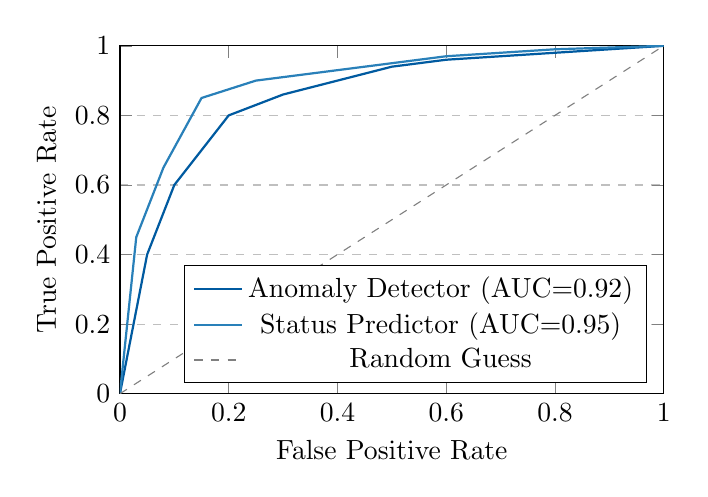
\begin{tikzpicture}
    \begin{axis}[
        width=\textwidth*0.7,
        height=6cm,
        xlabel={False Positive Rate},
        ylabel={True Positive Rate},
        xmin=0, xmax=1,
        ymin=0, ymax=1,
        xtick={0,0.2,0.4,0.6,0.8,1.0},
        ytick={0,0.2,0.4,0.6,0.8,1.0},
        legend pos=south east,
        ymajorgrids=true,
        grid style=dashed,
      ]
      
      \addplot[
        color=mainblue,
        thick,
        ]
        coordinates {
        (0, 0) (0.05, 0.4) (0.1, 0.6) (0.2, 0.8) (0.3, 0.86)
        (0.4, 0.9) (0.5, 0.94) (0.6, 0.96) (0.7, 0.97) (0.8, 0.98) (0.9, 0.99) (1.0, 1.0)
        };
      \addlegendentry{Anomaly Detector (AUC=0.92)}
      
      \addplot[
        color=secondaryblue,
        thick,
        ]
        coordinates {
        (0, 0) (0.03, 0.45) (0.08, 0.65) (0.15, 0.85) (0.25, 0.9)
        (0.4, 0.93) (0.5, 0.95) (0.6, 0.97) (0.7, 0.98) (0.8, 0.99) (0.9, 0.995) (1.0, 1.0)
        };
      \addlegendentry{Status Predictor (AUC=0.95)}
      
      \addplot[dashed, gray] coordinates {(0,0) (1,1)};
      \addlegendentry{Random Guess}
      
    \end{axis}
  \end{tikzpicture}
  \caption{ROC curves for classification models}
  \label{fig:roc_curves}
\end{figure}

\clearpage
\section{Visualization and Dashboards}

\subsection{Sensor Overview Dashboard}
The main dashboard provides a comprehensive view of all sensors:

\begin{figure}[H]
  \centering
  \fbox{\includegraphics[width=0.95\textwidth]{figures/sensor_dashboard.png}}
  \caption{Sensor overview dashboard showing real-time metrics and status}
  \label{fig:dashboard}
\end{figure}

Dashboard components include:
\begin{itemize}[leftmargin=*]
  \item Real-time temperature and humidity readings with thresholds
  \item Interactive geolocation heat map of sensor network
  \item Anomaly indicators with severity levels
  \item Historical trend analysis with comparison to predictions
\end{itemize}

\subsection{Anomaly Detection Visualization}
The anomaly dashboard highlights unusual patterns:

\begin{figure}[H]
  \centering
  \fbox{\includegraphics[width=0.95\textwidth]{figures/anomaly_dashboard.png}}
  \caption{Anomaly detection visualization with ML-based indicators}
  \label{fig:anomaly}
\end{figure}

Anomaly visualization features:
\begin{itemize}[leftmargin=*]
  \item Time series visualization highlighting anomalous points
  \item Probability distribution analysis of sensor readings
  \item Correlation explorer showing relationships between anomalies and environmental factors
  \item Alert history with detailed investigation tools
\end{itemize}

\clearpage
\section{Conclusion}
The Distributed ML Platform successfully demonstrates the integration of streaming, distributed processing, and machine learning for real-time sensor analytics. Key achievements include:

\begin{itemize}[leftmargin=*]
  \item A horizontally scalable architecture processing 700+ messages/second
  \item High-accuracy ML models with sub-15ms inference times
  \item End-to-end latency consistently below 300ms
  \item Interactive visualization dashboards providing actionable insights
\end{itemize}

\subsection{Lessons Learned}
During implementation, several important insights emerged:
\begin{itemize}[leftmargin=*]
  \item Proper Kafka partition sizing is crucial for optimal throughput
  \item Spark's micro-batch processing introduces a latency-throughput tradeoff
  \item ML model complexity significantly impacts overall system performance
  \item Elasticsearch indexing throughput requires careful tuning of refresh intervals
\end{itemize}

\subsection{Future Work}
Several enhancements could further improve the platform:
\begin{itemize}[leftmargin=*]
  \item Implementing online learning for continuous model improvement
  \item Extending to multi-cluster deployment for geographic distribution
  \item Incorporating federated learning for edge device integration
  \item Adding natural language processing for alert contextualization
\end{itemize}

\begin{figure}[h]
  \centering
  \fbox{\includegraphics[width=0.7\textwidth]{figures/conclusion.png}}
  \caption{System performance visualization across different workloads}
  \label{fig:conclusion}
\end{figure}

\clearpage
\begin{thebibliography}{9}
\bibitem{kafka} 
Kreps, J., Narkhede, N., Rao, J. (2011). 
\textit{Kafka: a distributed messaging system for log processing}. 
NetDB.

\bibitem{spark} 
Zaharia, M., Chowdhury, M., Franklin, M.J., Shenker, S., Stoica, I. (2010). 
\textit{Spark: Cluster Computing with Working Sets}. 
HotCloud.

\bibitem{structured_streaming} 
Armbrust, M., Das, T., Torres, J., Yavuz, B., Zhu, S., Xin, R., ... \& Zaharia, M. (2018). 
\textit{Structured Streaming: A Declarative API for Real-Time Applications in Apache Spark}. 
SIGMOD.

\bibitem{elasticsearch} 
Gormley, C., \& Tong, Z. (2015). 
\textit{Elasticsearch: The Definitive Guide: A Distributed Real-Time Search and Analytics Engine}.
O'Reilly Media.

\bibitem{mllib} 
Meng, X., Bradley, J., Yavuz, B., Sparks, E., Venkataraman, S., Liu, D., ... \& Talwalkar, A. (2016).
\textit{MLlib: Machine Learning in Apache Spark}.
Journal of Machine Learning Research, 17(34), 1-7.
\end{thebibliography}

\end{document}